% Asset 24 — rule-based programming vs machine learning, on one canvas.
% Left: a person writes the rules (the classic "rules + data -> answers"),
% drawn as the hand-written decision chart a programmer would produce for
% penguins. Right: machine learning ("data + answers -> rules"), with BOTH
% kinds of learning — supervised and unsupervised — on the same side.
\documentclass[border=10pt]{standalone}
% Shared preamble for every TikZ diagram in the workshop.
% Included by each asset file with % Shared preamble for every TikZ diagram in the workshop.
% Included by each asset file with % Shared preamble for every TikZ diagram in the workshop.
% Included by each asset file with \input{_preamble}.
%
% Compiled with lualatex so the diagrams use the SAME Inter typeface as the
% slides and the Manim clips. Falls back to the default sans if Inter is not
% installed, so a missing font degrades rather than fails.
\usepackage{iftex}
\ifLuaTeX
  \usepackage{fontspec}
  \IfFontExistsTF{Inter}{%
    \setsansfont{Inter}[
      UprightFont = *-Regular,
      BoldFont    = *-Bold,
      ItalicFont  = *-Italic,
      Extension   = .otf,
    ]%
  }{}
\fi
\renewcommand{\familydefault}{\sfdefault}

\usepackage{amsmath}
\usepackage{tikz}
\usetikzlibrary{positioning,arrows.meta,shapes.geometric,fit,backgrounds,calc,
                matrix,decorations.pathreplacing,patterns}

% --- the shared palette. Blue always means the same thing. ---------------
\definecolor{navy}{HTML}{1B2A4A}     % structure
\definecolor{cblue}{HTML}{2E5CA8}    % class A / train
\definecolor{corange}{HTML}{E07A2C}  % class B / test
\definecolor{cteal}{HTML}{2A9D8F}    % accent
\definecolor{cgray}{HTML}{D9DCE1}    % inactive

\tikzset{
  every picture/.style={line width=0.9pt},
  % a plain labelled container
  box/.style={
    draw=navy, rounded corners=3pt, fill=white,
    minimum width=26mm, minimum height=11mm, align=center,
    text=navy, font=\small
  },
  % a cell in a grid / array / dataframe
  cell/.style={
    draw=navy, fill=white, minimum width=13mm, minimum height=9mm,
    align=center, text=navy, font=\small, inner sep=1pt
  },
  hdr/.style={cell, fill=navy, text=white, font=\scriptsize\bfseries},
  blue/.style={draw=cblue, fill=cblue!12, text=navy},
  orange/.style={draw=corange, fill=corange!14, text=navy},
  teal/.style={draw=cteal, fill=cteal!12, text=navy},
  gray/.style={draw=cgray!140, fill=cgray!35, text=navy},
  % arrows
  arr/.style={-{Stealth[length=3mm,width=2.2mm]}, draw=navy, line width=1pt},
  arrblue/.style={arr, draw=cblue},
  arrorange/.style={arr, draw=corange},
  % text
  capt/.style={text=navy, font=\footnotesize, align=center},
  % fill=white so an annotation that sits on a connector masks it
  % rather than being crossed out by it
  note/.style={text=navy!70, font=\scriptsize\itshape, align=center,
                fill=white, inner sep=2pt},
  ttl/.style={text=navy, font=\bfseries, align=center},
  mono/.style={text=cblue, font=\small\ttfamily},
}
.
%
% Compiled with lualatex so the diagrams use the SAME Inter typeface as the
% slides and the Manim clips. Falls back to the default sans if Inter is not
% installed, so a missing font degrades rather than fails.
\usepackage{iftex}
\ifLuaTeX
  \usepackage{fontspec}
  \IfFontExistsTF{Inter}{%
    \setsansfont{Inter}[
      UprightFont = *-Regular,
      BoldFont    = *-Bold,
      ItalicFont  = *-Italic,
      Extension   = .otf,
    ]%
  }{}
\fi
\renewcommand{\familydefault}{\sfdefault}

\usepackage{amsmath}
\usepackage{tikz}
\usetikzlibrary{positioning,arrows.meta,shapes.geometric,fit,backgrounds,calc,
                matrix,decorations.pathreplacing,patterns}

% --- the shared palette. Blue always means the same thing. ---------------
\definecolor{navy}{HTML}{1B2A4A}     % structure
\definecolor{cblue}{HTML}{2E5CA8}    % class A / train
\definecolor{corange}{HTML}{E07A2C}  % class B / test
\definecolor{cteal}{HTML}{2A9D8F}    % accent
\definecolor{cgray}{HTML}{D9DCE1}    % inactive

\tikzset{
  every picture/.style={line width=0.9pt},
  % a plain labelled container
  box/.style={
    draw=navy, rounded corners=3pt, fill=white,
    minimum width=26mm, minimum height=11mm, align=center,
    text=navy, font=\small
  },
  % a cell in a grid / array / dataframe
  cell/.style={
    draw=navy, fill=white, minimum width=13mm, minimum height=9mm,
    align=center, text=navy, font=\small, inner sep=1pt
  },
  hdr/.style={cell, fill=navy, text=white, font=\scriptsize\bfseries},
  blue/.style={draw=cblue, fill=cblue!12, text=navy},
  orange/.style={draw=corange, fill=corange!14, text=navy},
  teal/.style={draw=cteal, fill=cteal!12, text=navy},
  gray/.style={draw=cgray!140, fill=cgray!35, text=navy},
  % arrows
  arr/.style={-{Stealth[length=3mm,width=2.2mm]}, draw=navy, line width=1pt},
  arrblue/.style={arr, draw=cblue},
  arrorange/.style={arr, draw=corange},
  % text
  capt/.style={text=navy, font=\footnotesize, align=center},
  % fill=white so an annotation that sits on a connector masks it
  % rather than being crossed out by it
  note/.style={text=navy!70, font=\scriptsize\itshape, align=center,
                fill=white, inner sep=2pt},
  ttl/.style={text=navy, font=\bfseries, align=center},
  mono/.style={text=cblue, font=\small\ttfamily},
}
.
%
% Compiled with lualatex so the diagrams use the SAME Inter typeface as the
% slides and the Manim clips. Falls back to the default sans if Inter is not
% installed, so a missing font degrades rather than fails.
\usepackage{iftex}
\ifLuaTeX
  \usepackage{fontspec}
  \IfFontExistsTF{Inter}{%
    \setsansfont{Inter}[
      UprightFont = *-Regular,
      BoldFont    = *-Bold,
      ItalicFont  = *-Italic,
      Extension   = .otf,
    ]%
  }{}
\fi
\renewcommand{\familydefault}{\sfdefault}

\usepackage{amsmath}
\usepackage{tikz}
\usetikzlibrary{positioning,arrows.meta,shapes.geometric,fit,backgrounds,calc,
                matrix,decorations.pathreplacing,patterns}

% --- the shared palette. Blue always means the same thing. ---------------
\definecolor{navy}{HTML}{1B2A4A}     % structure
\definecolor{cblue}{HTML}{2E5CA8}    % class A / train
\definecolor{corange}{HTML}{E07A2C}  % class B / test
\definecolor{cteal}{HTML}{2A9D8F}    % accent
\definecolor{cgray}{HTML}{D9DCE1}    % inactive

\tikzset{
  every picture/.style={line width=0.9pt},
  % a plain labelled container
  box/.style={
    draw=navy, rounded corners=3pt, fill=white,
    minimum width=26mm, minimum height=11mm, align=center,
    text=navy, font=\small
  },
  % a cell in a grid / array / dataframe
  cell/.style={
    draw=navy, fill=white, minimum width=13mm, minimum height=9mm,
    align=center, text=navy, font=\small, inner sep=1pt
  },
  hdr/.style={cell, fill=navy, text=white, font=\scriptsize\bfseries},
  blue/.style={draw=cblue, fill=cblue!12, text=navy},
  orange/.style={draw=corange, fill=corange!14, text=navy},
  teal/.style={draw=cteal, fill=cteal!12, text=navy},
  gray/.style={draw=cgray!140, fill=cgray!35, text=navy},
  % arrows
  arr/.style={-{Stealth[length=3mm,width=2.2mm]}, draw=navy, line width=1pt},
  arrblue/.style={arr, draw=cblue},
  arrorange/.style={arr, draw=corange},
  % text
  capt/.style={text=navy, font=\footnotesize, align=center},
  % fill=white so an annotation that sits on a connector masks it
  % rather than being crossed out by it
  note/.style={text=navy!70, font=\scriptsize\itshape, align=center,
                fill=white, inner sep=2pt},
  ttl/.style={text=navy, font=\bfseries, align=center},
  mono/.style={text=cblue, font=\small\ttfamily},
}

\begin{document}
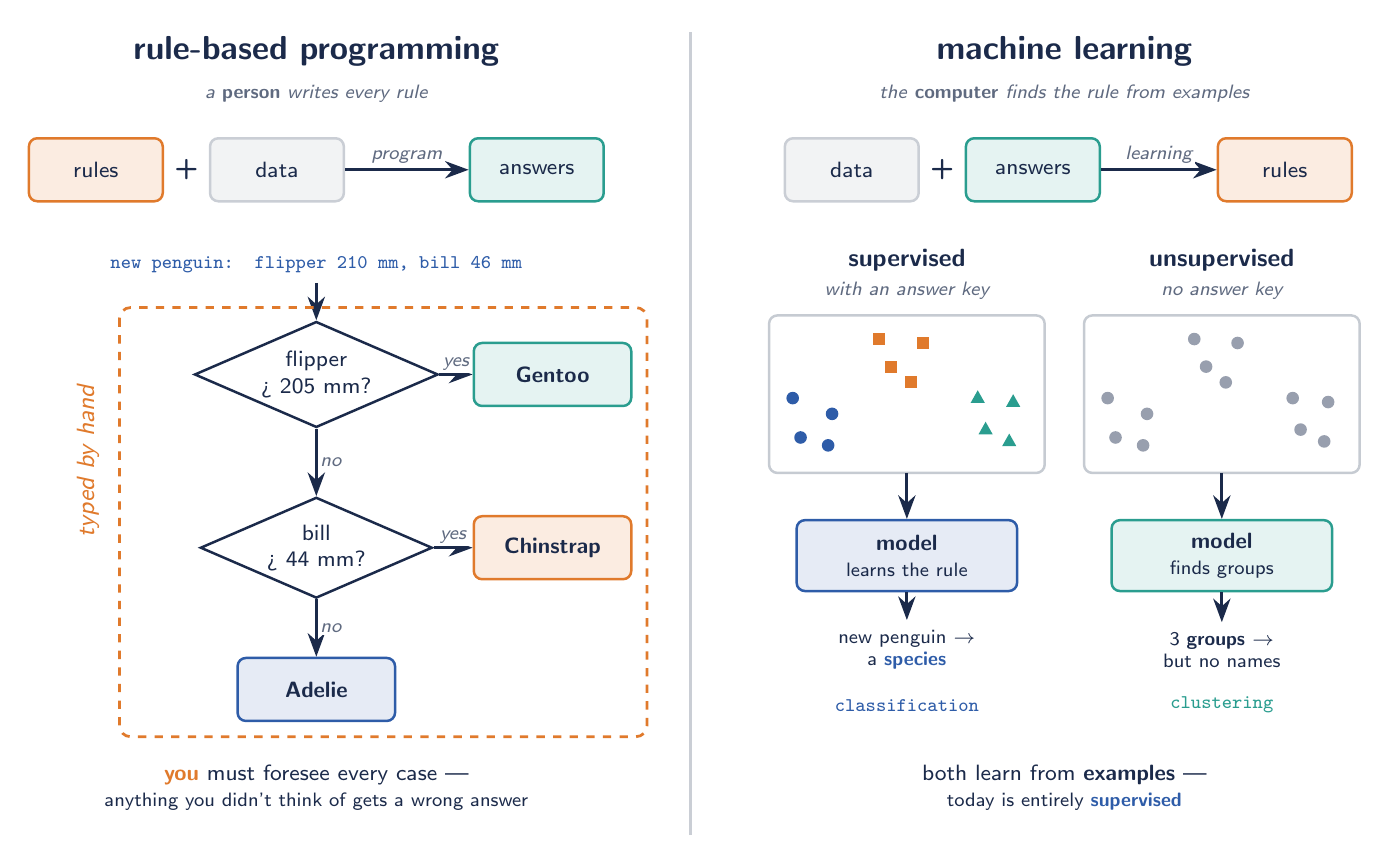
\begin{tikzpicture}[
  sm/.style={box, minimum width=17mm, minimum height=8mm, font=\footnotesize},
  q/.style={diamond, aspect=2.3, draw=navy, fill=white, text=navy,
            font=\footnotesize, inner sep=1.5pt, align=center},
  ans/.style={box, minimum width=20mm, minimum height=8mm, font=\footnotesize\bfseries},
  yn/.style={text=navy!70, font=\scriptsize\itshape, fill=white, inner sep=1pt},
]

% ======================= LEFT: RULE-BASED =======================
\node[ttl] at (-4.75,5.25) {\large rule-based programming};
\node[note] at (-4.75,4.72) {a \textbf{person} writes every rule};

\node[sm, orange] (lr) at (-7.55,3.75) {rules};
\node[text=navy] at (-6.4,3.75) {\textbf{+}};
\node[sm, gray]  (ld) at (-5.25,3.75) {data};
\node[sm, teal]  (la) at (-1.95,3.75) {answers};
\draw[arr] (ld.east) -- node[yn, above=1pt] {program} (la.west);

% the hand-written decision chart
\node[mono, font=\scriptsize\ttfamily] (pen) at (-4.75,2.55)
     {new penguin: flipper 210 mm, bill 46 mm};
\node[q] (q1) at (-4.75,1.15) {flipper\\> 205 mm?};
\node[ans, teal]   (g) at (-1.75,1.15) {Gentoo};
\node[q] (q2) at (-4.75,-1.05) {bill\\> 44 mm?};
\node[ans, orange] (c) at (-1.75,-1.05) {Chinstrap};
\node[ans, blue]   (a) at (-4.75,-2.85) {Adelie};

\draw[arr] (pen.south) -- (q1.north);
\draw[arr] (q1.east) -- node[yn, above] {yes} (g.west);
\draw[arr] (q1.south) -- node[yn, right] {no} (q2.north);
\draw[arr] (q2.east) -- node[yn, above] {yes} (c.west);
\draw[arr] (q2.south) -- node[yn, right] {no} (a.north);

\node[note, rotate=90, text=corange] at (-7.65,0.05) {\small typed by hand};
\draw[corange, line width=1pt, rounded corners=4pt, dashed]
      (-7.25,2.0) rectangle (-0.55,-3.45);

\node[capt, align=center] at (-4.75,-4.1)
     {\textcolor{corange}{\textbf{you}} must foresee every case ---\\
      \scriptsize anything you didn't think of gets a wrong answer};

% divider
\draw[cgray!140, line width=1pt] (0,-4.7) -- (0,5.5);

% ======================= RIGHT: MACHINE LEARNING =======================
\node[ttl] at (4.75,5.25) {\large machine learning};
\node[note] at (4.75,4.72) {the \textbf{computer} finds the rule from examples};

\node[sm, gray]  (rd) at (2.05,3.75) {data};
\node[text=navy] at (3.2,3.75) {\textbf{+}};
\node[sm, teal]  (ra) at (4.35,3.75) {answers};
\node[sm, orange] (rr) at (7.55,3.75) {rules};
\draw[arr] (ra.east) -- node[yn, above=1pt] {learning} (rr.west);

% --- supervised (left of the right half)
\node[ttl, font=\small\bfseries] at (2.75,2.6) {supervised};
\node[note] at (2.75,2.22) {with an answer key};
\draw[cgray!150, rounded corners=3pt] (1.0,-0.1) rectangle (4.5,1.9);
\foreach \x/\y in {1.4/0.35, 1.8/0.65, 1.3/0.85, 1.75/0.25} \fill[cblue] (\x,\y) circle (0.08);
\foreach \x/\y in {2.55/1.25, 2.95/1.55, 2.4/1.6, 2.8/1.05}
  \fill[corange] ($(\x,\y)+(-0.075,-0.075)$) rectangle ++(0.15,0.15);
\foreach \x/\y in {3.75/0.45, 4.1/0.8, 3.65/0.85, 4.05/0.3}
  \fill[cteal] ($(\x,\y)+(0,0.1)$) -- ++(0.09,-0.16) -- ++(-0.18,0) -- cycle;
\node[box, blue, minimum width=28mm, minimum height=9mm, font=\footnotesize] (sm) at (2.75,-1.15)
     {\textbf{model}\\\scriptsize learns the rule};
\draw[arr] (2.75,-0.1) -- (sm.north);
\node[capt, align=center, font=\scriptsize] (sout) at (2.75,-2.35)
     {new penguin $\rightarrow$\\a \textcolor{cblue}{\textbf{species}}};
\draw[arr] (sm.south) -- (sout.north);
\node[mono, font=\scriptsize\ttfamily] at (2.75,-3.05) {classification};

% --- unsupervised (right of the right half)
\node[ttl, font=\small\bfseries] at (6.75,2.6) {unsupervised};
\node[note] at (6.75,2.22) {no answer key};
\draw[cgray!150, rounded corners=3pt] (5.0,-0.1) rectangle (8.5,1.9);
\foreach \x/\y in {5.4/0.35, 5.8/0.65, 5.3/0.85, 5.75/0.25,
                   6.55/1.25, 6.95/1.55, 6.4/1.6, 6.8/1.05,
                   7.75/0.45, 8.1/0.8, 7.65/0.85, 8.05/0.3}
  \fill[navy!45] (\x,\y) circle (0.08);
\node[box, teal, minimum width=28mm, minimum height=9mm, font=\footnotesize] (um) at (6.75,-1.15)
     {\textbf{model}\\\scriptsize finds groups};
\draw[arr] (6.75,-0.1) -- (um.north);
\node[capt, align=center, font=\scriptsize] (uout) at (6.75,-2.35)
     {3 \textbf{groups} $\rightarrow$\\\scriptsize but no names};
\draw[arr] (um.south) -- (uout.north);
\node[mono, font=\scriptsize\ttfamily, text=cteal] at (6.75,-3.05) {clustering};

\node[capt, align=center] at (4.75,-4.1)
     {both learn from \textbf{examples} ---\\
      \scriptsize today is entirely \textcolor{cblue}{\textbf{supervised}}};

\end{tikzpicture}
\end{document}
